\chapter{绪\quad 论}

\section{多核系统概述}
20世纪90年代,随着商业化微处理器的生产成本的降低,计算机处理器设计人员开始寻求性能强于单个微处理器的用于构建服务器和超级计算机的多处理器。
伴随着单处理器上性能的增幅减少以及对计算机功耗的关注,促成了人们热衷于研究指令级并行(ILP)技术,这致使计算机体系结构进入新的时代——一个多处理器在低端到高端市场扮演主要角色的时代。

\subsection{多核体系结构}
多处理技术的重要性体现在以下几个方面:
\begin{itemize}
	\item 2000年至2005年期间,研究人员在寻找和利用更高的指令级并行期间发现,功耗和硅成本的增长速度远超性能增长的速度,更高的指令级并行理论意义大于实际意义。除了指令级并行之外,另一条为人熟知的可能比基础技术具有更高性能的方法便是通过多处理(Multiprocessing)。
	\item 云计算和软件即服务(saas)对高端服务器的需求越来越大;
	\item 互联网上的海量数据刺激数据密集型应用的增长;
	\item 有观点认为提升桌面电脑性能相比之下不再那么重要(至少在图形处理方面),要么是因为当前的桌面电脑满足性能需求,要么是因为高强度的计算密集型和数据密集型应用可以通过云计算完成。
	\item 人们对于如何有效的使用多处理器的认识的加深。
\end{itemize}

处理器是指计算机系统中的中央处理单元(CPU)。
它由多级指令和数据缓存、指令译码器和不同类型的算术和逻辑运算单元构成。
多处理器是指由多个紧密耦合的处理器构成的计算机系统,多个处理器的协调和使用受同一个操作系统控制,并通过共享地址空间共享内存\cite{hennessy2011computer}。

计算机系统为了增强性能,降低功耗以及更加有效的同时处理多任务,将两个或两个以上用于读取和执行程序指令的独立处理单元(通常被称为核心)集成到CPU芯片上,这种集成了多个计算核心的芯片被称为\textbf{片上多核处理器(Chip Multi-core Processor)}\cite{geer2005chip}。
每个核心都具有单独的一级缓存和执行单元,同一个处理器上的所有核心共享二级缓存。
这种设计意味着虽然处理器有一个相比之下容量更大的缓存池,但每个核心拥有访问速度更快的内存空间和算术/逻辑运算单元。
因此,单个处理器可以在不同的核心上同时运行多个指令,这种处理方式被称为芯片级多处理(Chip-level Multiprocessing)。

更细一步的划分,一个核内可以同时执行多个线程,这种同时执行的线程被称为\textbf{同步多线程}(Simultaneous Multithreading,简称SMT),也叫同时多线程。
尽管多个线程运行在相同的核心内,但线程之间是完全隔离开的。
同步多线程是多线程的两个主要实现之一,另一个是时间多线程(也称超线程)。
在同步多线程中,多于一个线程的指令可以在任何指定的流水线阶段中同时执行。
实现同步多线程技术在基本的处理器架构上进行修改:一是增加了在一个周期中从多个线程获取指令的能力;二是设置一个更大的寄存器文件用于保存来自多个线程的数据。
核心支持的并发线程的数量可以由芯片设计者决定。
Intel超线程技术(Hyper-threading)就是SMT实现的一个典型技术\cite{marr2002hyper}。
最新款英特尔Core vPro处理器系列\cite{samson2005interface}、Core处理器系列\cite{lempel20112nd}、Core M处理器系列和Xeon处理器系列\cite{chang200765}都采用了英特尔超线程技术。
常见模式是每个CPU核心支持两个并发线程,Sun公司2004年推出的第一款SPARC架构的多核处理器UltraSPARC T1 Niagara每个核心支持4个同步线程\cite{kongetira2005niagara},后续推出的Niagara2每个核心支持8个同步线程。

为了充分利用发挥具有$n$个处理器的多指令多数据(MIMD)多处理器的优势,系统中必须要有至少$n$个线程或进程。
单个进程中的独立线程通常是由程序员标识出来或者通过操作系统创建。
分配给线程的计算量(称为粒度)在考虑如何有效利用线程级并行性方面很重要,线程级并行与指令级并行的重要的本质区别在于线程级并行性由高层 软件系统或程序员标识,并且线程由数百到数百万条可并行执行的指令组成。
线程也可以用来利用数据级的并行性,但是它的开销可能高于单指令多数据(SIMD)处理器或GPU\cite{shi2012vcuda}。
线程的高开销意味着要充分的发挥并行性它的粒度必须足够大。

共享内存多处理器(Shared Memroy Multiprocessor)是一种典型的多处理器系统架构。
共享内存多处理器在智能移动终端、服务器上的普及带来了并发编程技术上的重大变化。
随着支持多线程的芯片的成本的降低以及单处理器无法突破现有的性能瓶颈,配备多处理器的计算机设备会变得越来越普遍。
系统中包含的处理器的数量不同,决定了处理器间的内存组织方式和互联策略的差异,因此,按照处理器的内存组织方式可以将现有的共享内存多处理器分为两类:第一类为\textbf{对称多处理器(Symmetric (shared-memory) Multiprocessors,简称SMPs)},又称为集中式共享内存多处理器。
	这种结构的处理器特点是具有少量的处理器,通常为8个或者更少。
	对于具有如此小的处理器数量的多处理器,所有处理器可以共享一个单一的集中存储器,所有处理器都有相同的访问权限,“对称”因此得名。
	在每一块多核芯片上,核心之间的内存都采用共享的方式。当前连接的多核芯片的数量大于1时,会为每一块芯片分配单独的内存,此时的内存是分布式的。SMP体系结构的处理器通常也称\textbf{统一的内存访问(Uniform Memory Access,简称UMA)多处理器},这是因为所有的处理器都具有相同的内存延迟。图~\ref{fig:uma}所示为SMP体系结构的多处理器结构图。
	处理器的缓存子系统共享相同的物理内存,通常情况下具有一级共享内存,每个处理器内的核心具有一级或多级的私有缓存。该架构的重要属性是,所有的处理器具有相同的内存访问时间跟延迟。
	所有的处理器都必须通过一条总线实现同步与内存访问,因此,统一内存访问架构的多处理器系统的最大性能瓶颈是内存。
	当系统的处理器个数大于32时,因为总线争用将十分激烈,严重影响多核系统性能使用单总线连接处理器和内存模块的方式不可取。
\begin{figure}
\centering
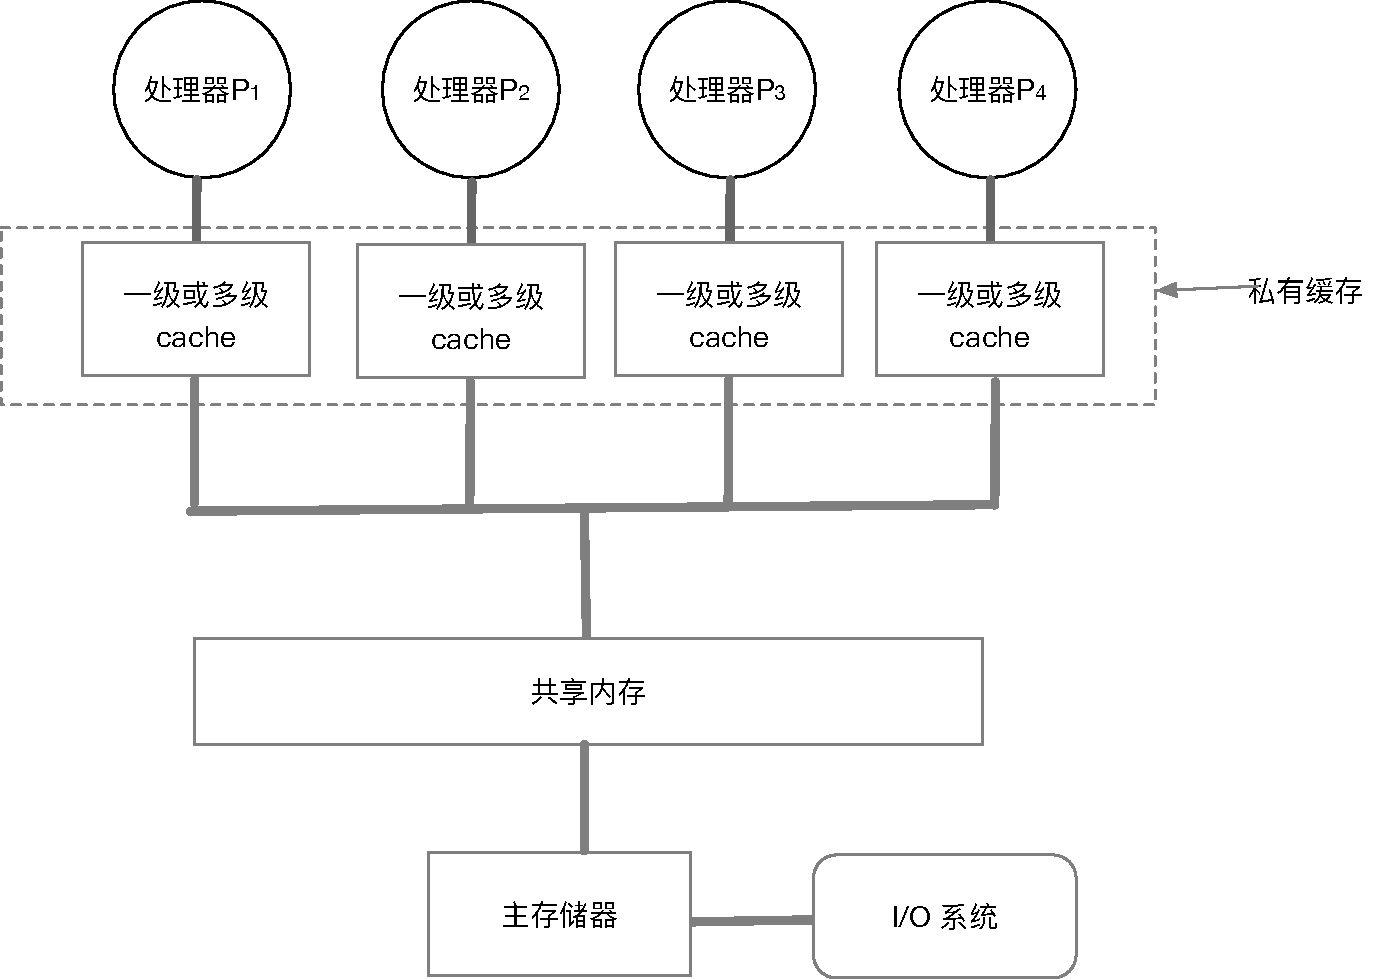
\includegraphics[width=0.65\textwidth]{uma}
\caption{SMP架构多处理器的基本结构示意图}
\label{fig:uma}
\end{figure}
	
	当系统内的处理器数量较多时,使用SMP架构会对系统性能造成影响,因此处理器数量较多的系统通常采用第二种架构:\textbf{分布式共享内存(Distributed Shared Memory,简称DSM)}架构。
	DSM是与SMP相对的一种体系结构,这种架构的多处理器共享逻辑地址空间,但是物理内存是分布式的。
	图~\ref{fig:dsm}所示为DSM体系结构多处理器的结构简图。
	为了支持更大的处理器数量,系统的内存必须是分布式的。
	否则,内存系统无法在保持内存访问延迟较低的前提下满足大量处理器的内存带宽需求。
	随着处理器性能的快速增加以及随之增长的内存带宽的需求,分布式内存要求的多处理器的规模将持续缩小。
	将内存分布在不同的结点上不仅增加了内存带宽,同时也满足了处理器访问内存低延迟的要求。
	由于访问时间取决于数据在本地内存结点还是远程内存结点上,因此,DSM多处理器通常也被称为\textbf{非一致内存体系结构(Non Uniform Memory Architecture,简称NUMA)}多处理器。DSM的主要缺点是处理器之间的数据传输更加复杂,若要充分利用分布式存储器提供的更高的内存带宽需要花费更多的精力进行软件设计。

在SMP和DSM两种体系结构的多处理器中,线程之间的通信都是通过共享地址空间进行的,这意味着只要处理器具有必要的访问权限,任何处理器都可以在任何内存位置上进行内存引用。
与SMP和DSM相关的术语\textbf{共享内存}是指地址空间是共享的。

\begin{figure}
\centering
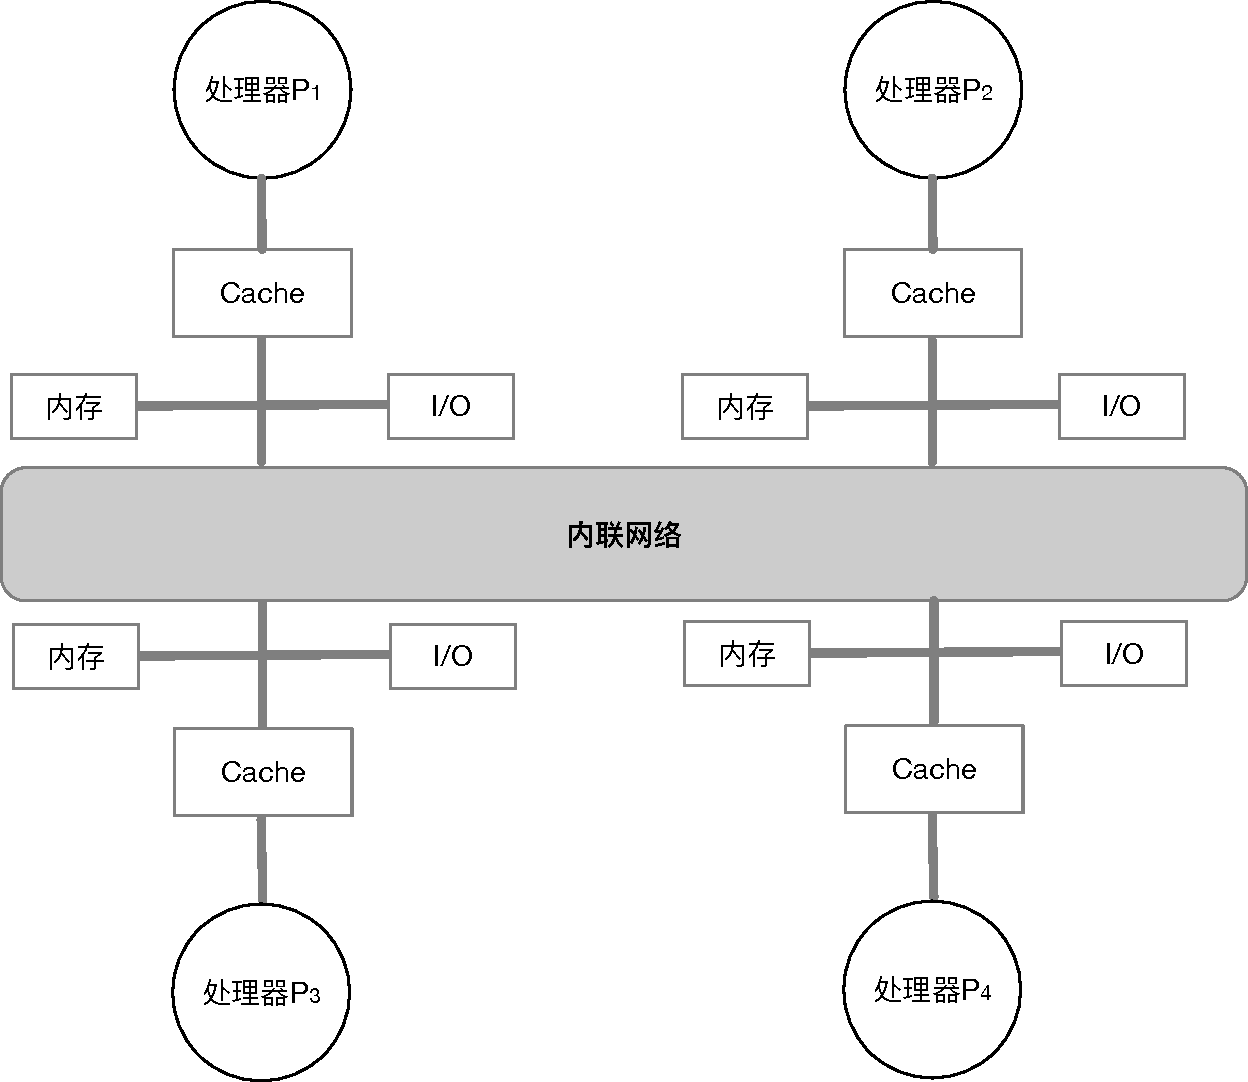
\includegraphics[width=0.65\textwidth]{dsm}
\caption{DSM架构多处理器结构示意图}
\label{fig:dsm}
\end{figure}


如果每个处理器上都具有一个调度器使系统上的多个CPU可以并行的执行任务。
这样的处理器系统被称为对称多处理(symmetric multiprocessing,简称SMP)系统。

负载均衡是多处理器系统的一个显著特点。
如果内核上的进程分布不均衡,即便是系统中的处理器数量再多,对于性能的提升也是微乎其微的。
对称多处理器系统实现负载均衡有两种途径:
第一种方法是将“准备就绪”的进程插入到一个可以共用进程队列中,每个处理器上的调度器都能访问这个进程队列。
当某个处理器中的调度器被激活时,它将从“准备就绪”的进程队列中选取一个进程进入处理器进行运算。
对称多处理系统通过使用共用的“准备就绪”的进程队列实现负载自动均衡。
当某个处理器为空闲状态时,它的调度器会从队列中选取一个进程,并开始在该处理器上运行。
这种方法能够实现处理器负载的自动均衡,但是共用的进程队列实现较为困难。

因此,为SMP设计的现代操作系统通常为每个处理器分配一个进程队列。
这种操作系统使用显示的负载均衡机制,通过这个机制,过载的处理器上的等待列表中的进程会被移动到另外的负载较少的处理器的进程队列中。
例如,SMP Linux系统每间隔200毫秒就激活一次负载均衡机制\cite{bolla2008effective}。
这种方法也存在一个问题,当每个核心都具有私有缓存时,将进程迁移到不同的处理器上的代价高昂。
因此一些操作系统(如Linux)提供一个系统调用来指定与处理器绑定的进程,这与处理器负载无关。

\textbf{多核处理器和多处理器的区别与联系}:多核处理器是指一个CPU内包含若干个计算单元;而多处理器是指在计算机内存在多个相同的CPU。
以双核处理器为例,双核心的设置类似于在同一台计算机上安装两个独立的处理器,但是由于两个核心实际上位于同一块芯片上,它们之间的信息交换的速度要快于同一台计算机上的两个独立的处理器之间的通信速度。
多处理器的CPU可以是由多个普通的只具有一个核心的CPU构成,也可以是由多个多核CPU构成。

在本文的研究中,使用的五个实验平台的其中四个是基于NUMA架构的多处理器系统,另外一个是Intel的基于Many Integrated Core(MIC)架构的众核处理器。

\subsection{多核系统的缓存一致性}
多核系统的体系结构决定了它的缓存系统的复杂性。
在大多数现代多核系统上,每个处理器核心都具有独立的一级私有缓存,同一个CPU内的多个核心共享二级缓存。
当系统只有一个核心工作时,数据的一致性是能够保障的,一旦系统上有多个核心同时工作,就会出现缓存一致性问题。
试想当某个CPU $c_1$缓存行中对应的内存内容被另一个CPU $c_2$做了修改,而$c_1$没有收到任何关于该内容被修改的通知,那么$c_1$在下一次读取该数据的时候获取的是一个错误的值,从而导致运算结果偏离预期。
这种后果往往是灾难性的。
因此,在拥有多组缓存的情况下,保持这些缓存数据的同步至关重要,这需要设计一种各个缓存都能遵守的协议来实现同步。

注意到造成缓存不一致的根源问题在于系统拥有多组缓存,而不是因为系统拥有多个处理器核心。
一种直观的解决方案是让多个处理器核心共用一组缓存,即只设计一块一级缓存。
在任何一个指令周期内,只有一个处理器核心能够通过一级缓存进行内存操作,完成其相应的指令。
这在逻辑上没有任何问题,唯一的问题是效率太低。
所有的核心都需要排队等待使用一级缓存。
最终问题还是要回到使用多组缓存上来,但要设法让多组缓存之间的行为看上去就像只有一组缓存在工作一样。
缓存一致性协议便在这样的背景下应运而生。

缓存一致性协议有多种,常见的计算机设备上使用的是基于“窥探(snooping)”协议。
它的基本思想是所有内存传输都发生在一条共享的总线上,而这条总线对所有的处理器都是可见的,缓存不仅在做内存传输时才和总线打交到,而是不同地在窥探总线上发生的数据交换,跟踪其它缓存在做什么。
这种协议的好处是延迟低。
但是这种总线型的设计方式不适合大规模的多核处理器系统。
在大规模的多处理器系统上使用的是“基于目录的(directory-based)”协议。
使用这种机制的缓存一致性协议的弊端是延迟较高,但是具有较好的可扩展性。

现代的多核处理器使用的缓存一致性协议为MESI协议及其衍生协议。
MESI协议得名于该协议约定的四种缓存行状态:已修改(Modified),独占(Exclusive),共享(Shared)和失效(Invalid)的首字母。
为了叙述的方便起见,本文将以相反的顺序对这四种状态进行描述:
\begin{itemize}
	\item I是指该缓存行要么已经被替换出了缓存,要么是该缓存行上存储的内容已经过时。
	为了达到缓存的目的,处理器读取缓存行数据时,被标记为I的缓存行会被忽略。
	也就是说,一旦缓存行被标记为失效,等同于该缓存行未被加载进缓存内。
	\item S表明该缓存行存储的内容是与主存内容一致的一份副本,处于S状态的缓存行只能被读取,不能进行写入。
	多组缓存可以同时拥有来自同一内存地址的共享缓存行。
	\item E状态的缓存行与S状态的一样,也是和主存内容一致的一份副本。
	区别在于如果一个处理器持有了某个E状态的缓存行,那么其它的处理器就不能同时持有它,这就是名字“独占”的由来。
	这意味着如果其它处理器原本也持有同一缓存行,则该处理器持有的缓存行马上会转变成I状态。
	\item M状态的缓存行,属于脏(dirty)缓存行,表明它已经被持有它的处理器修改了。
	如果一个缓存行处于M状态,那么它在其它处理器缓存中的副本马上就会转变成I状态,这个规律与E状态对副本的处理一样。
	此外,已修改的缓存行如果被替换出缓存或被标记为I状态,那么先要将它的内容回写到主存中。
\end{itemize}

将上述四种状态和单核系统中回写模式的缓存对比,发现状态I、S和M都有对应的概念:失效/未载入、干净以及脏的缓存行。
这里唯一没有对应的是E状态,代表某个处理器的独占访问权限。
这个状态解决了“在对某块内存进行修改之前通知其它处理器”的问题。
当处理器想对某个缓存行进行写入时,如果它没有独占权,它必须先发送一条请求独占的请求给总线,然后广播其它处理器,使它们拥有的同一缓存行的副本失效。
反之,如果其它处理器想读取这个缓存行,M或者E状态的缓存行必须先回到S状态。
如果是M状态的缓存行,还需要先将更新的内容回写到主存中。

在进行多核系统的软件开发时,需要理解两点:

第一,在多核系统中,读取某个缓存行,实际上会牵涉到和其他处理器的通讯,并且可能导致它们发生内存传输。
写某个缓存段需要多个步骤:在写入数据之前,首先要获得独占权,以及所请求的缓存行的当前内容的拷贝。

第二,尽管系统为了保障缓存一致性做了许多复杂的工作,但是最终的结果还是能够保证的。
它遵循MESI定律\cite{Fabian-ryg}——在所有的脏缓存行(M状态)被回写后,任意缓存级别的所有缓存行中的内容,和它们对应的内存中的内容一致。此外,在任意时刻,当某个位置的内存被一个处理器加载入独占缓存行时(E状态),那它就不会再出现在其他任何处理器的缓存中。

在原生的MESI协议的基础上,衍生出了MOSEI,MESIF等变种。
MOSEI协议的“O”(Owned)状态与E状态类似,也是保证缓存键一致性的手段,但它直接共享脏的缓存行的内容,而不需要先把脏缓存行回写到内存中。
这种协议用于AMD Opteron处理器上。
MESIF协议扩展了一个“F”(Forward)状态,它制定某个处理器专门处理针对某个缓存行的读操作。当多个处理器同时拥有某个S状态的缓存行时,只有被指定的那个处理器(即对应的缓存行为F状态)才能对读操作做出回应。
这种设计可以降低总线的数据流量。Intel的大部分多核处理器采用MESIF协议。 

\section{课题研究背景及意义}

并发哈希表(CHT)是一种允许在同一时刻有多个读者或写者访问共享对象的哈希表。
其提供与串行哈希表一样的访问接口,但是CHT能够更有效的发挥多核处理器的性能。
对于所有并发数据结构而言,断言并发访问是一项必要工作。
在并发编程模型里基于锁和无锁是两种常用的同步控制方式,用于确保多个线程有序的对内存进行访问。
为了保证线程安全性,基于锁的并发哈希表对临界区进行加锁操作。锁的实现有粗、细两种不同的粒度。
粗粒度锁在实现上相对简单,但是采用粗粒度锁往往临界区特别长,阻碍对计算机资源的高效利用。
使用细粒度锁的好处是允许多个线程对数据的不同区段进行并发的读/写。
锁的粒度越细,越有利于提升整体性能,但是同时在实现和正确性验证上也需要耗费更多的精力。
另一种相对的并发编程范式是无锁。无锁化编程是用计算机原语来代替显示锁的一种并发编程范式。
此外还有使用非阻塞方法实现的并发哈希表\cite{nonblocking,clht,shalev2006split}。

\subsection{并发哈希表的性能评估}
 
对于并发哈希算法的评估指标主要包括:吞吐量;哈希表的线程扩展性;操作的延迟;内存使用情况;哈希表的空间利用率等方面。
吞吐量是指在单位时间内哈希表执行插入、删除、查询操作的总量,单位为Mops/s或者ops/ms。
线程扩展性是用来衡量运行在多处理器机器上的应用的效率的重要指标。
应用程序的线程扩展性是指随着程序启用的物理线程的数量的增加,应用的吞吐量保持不减的能力。
理想情况下程序的性能应该与物理线程的数量呈线性关系。
延迟是指平均每执行一次哈希表操作需要耗费的CPU时钟周期数。
内存使用情况是指处理同等规模的数据下,消耗的内存。
哈希表的空间利用率是指哈希表在不进行扩容操作的前提下性能达到饱和时,哈希表内实体的数量与哈希表存储能力的比值,在有些文献中哈希表的空间利用率也被称作负载因子(load factor)。

在现有的相关研究成果中\cite{clht,cuckoo,hopscotch,metreveli2012cphash,nonblocking},对哈希表进行评估时所使用的哈希表的设计方法、优化方案、内存分配与管理、测试环境、测试数据、性能评估指标等方面都存在出入。
设计方法上的差异体现在哈希函数的选取;采用什么样的冲突处理方法处理发生冲突的数据;采用哪种同步方法实现多个线程的并发访问。

Y.Liu等人设计了一种可动态调整哈希表大小的无阻塞并发哈希表\cite{nonblocking}。
他们的算法是基于Java的,都使用java.util.concurrent包进行优化。
他们对并发哈希表进行评估时选取使用了相同的冲突处理技术和类似同步方法的SplitOrder哈希表\cite{shalev2006split}的吞吐量曲线和线程扩展性曲线作为基准线,测试在两种不同的多核处理器架构上(X86和SPRAC)展开。
因为这类哈希表支持动态调整哈希表的大小,所以对于哈希表的空间利用率的评估意义不大。

Z.Metreveli等人设计了一种缓存分区哈希表——CPHash\cite{metreveli2012cphash},CPHash将查找/插入请求通过消息传递机制传输到指定的缓存分区内(分区的大小设置为缓存行的大小)。这种设计的目的有两个:一是使用消息传递机制替代传统的锁;二是采用批处理的方式避免过于频繁的缓存行切换。
所以对CPHash的性能评估侧重其与基于锁的同类哈希表的比较,突出消息传递机制取代锁方法的重要意义。

X.Li等人在传统的Cuckoo哈希表的基础上实现了支持多读多写的并发Cuckoo哈希表\cite{cuckoo}。
由于其独特的组相连设计,它的空间利用率是现有的并发哈希表中最好的之一。
Cuckoo哈希表对锁方法、内存消耗、Cuckoo查找路径都进行了优化,所以对于它的评估主要集中在吞吐量、内存消耗、哈希表的空间利用率等方面。

T.David等人对并发数据结构的评估方法相对来说是目前现有工作中最为全面的\cite{clht}。
他们通过对现有的一些并发数据结果的评估,总结了4条"异步并发(ASCY)"并发编程范式。
遵循这4条ASCY模式设计了缓存行哈希表(CLHT)。
缓存行哈希表的核心思想是对哈希表内的元素进行操作时尽量减少缓存行切换。
所以,对CLHT的评估重点在哈希表的线程扩展性、操作延迟、吞吐量等方面,没有针对硬件平台的特点进行优化。

从上述几种并发哈希表的评估方法中可以看出,现有的并发哈希表的评估方法都紧密围绕其设计方法展开的,这样的评估方法缺乏客观性:放大了自身方法优于其它方法的点,而选择性的隐藏自身方法中的性能瓶颈与问题。
这对并发哈希表的设计、优化、应用都是不利的。
用户无法直观判断在其应用中选择哪种并发哈希表能够获得更高的性能。

因此,设计一个统一的测试框架,为并发哈希表的评估提供公平的测试环境,排除因硬件特性、线程分配、内存管理、数据分布、数据集的差别等因素的影响,
充分从吞吐量、线程扩展性、内存消耗、同步方法、延迟、实现的难易程度等方面予以考察,确定设计和使用并发哈希表的最佳实践意义重大。

\subsection{并发哈希表的设计}
设计具有线程扩展性和充分利用处理器多核心优势的并发哈希表是一项富有挑战性的工作。
即使是在特定的平台上实现一个达到预期性能要求的具有可扩展性的并发哈希表也是具有相当难度的课题。
在某种体系结构上所采用的优化方法可能会在其他的体系结构上失去作用\cite{baumann2009multikernel,david}。
比如,针对NUMA架构的多处理器使用的优化方法对与SMP架构的系统就没有任何意义\cite{david}。
针对某种硬件特性使用的优化方案在不支持这种硬件指令的系统上甚至都无法实现正常编译。
比如使用RTM优化的并发哈希表在不支持RTM的机器上无法编译。
再者,如果某个并发哈希表是针对特定类型的工作集而进行的优化,那么工作集轻微的变化将造成性能的不稳定或者极速下降。
如使用RCU机制设计的并发哈希表,总所周知,RCU机制适合用于处理读占绝大多数的数据集,但是对于数据集中包含有更新操作的场景,使用这种即是实现的并发哈希表的性能甚至无法达到单个处理器系统的同类串行的哈希表\cite{urcu}。

本文的目标之一是要探究是否可以确定并发哈希表的特性。
确定这些特性有助于实现并发哈希表的\textit{可移植的扩展性},即在不同的平台、工作负载和性能指标上都具有扩展性。
乍一看,这个目标可能看起来很模糊,因为它提出了一个根本性的问题:在综合考虑数据结构、体系结构、性能指标和工作负载的前提条件下,我们可以期望获得具有哪种程度的扩展性?

% 实际上,根据特定的硬件特征和工作负载可以推算出所设计的并发哈希表的可扩展性的上界。
研究表明,对于现代的多核处理器而言,由对共享数据的存储操作引发的一致性流量是抑制并发软件可扩展性的最大障碍。
然而,受并发数据结构固有语义的限制,并发数据结构中不得不存在一定比例的存储操作,这些存储操作是无法省略或者被其他操作替换的;
通常在这些数据结构的串行版本中(即不支持多个进程共享的同种数据结构)也有相同的存储操作。
假设将这样的串行数据结构部署到多核系统上并且由多线程共享该数据结构,显然会得到错误的(如非线性化\cite{herlihy1990linearizability})执行结果。
然而,这种异步执行的程序的性能指明了如何对这些数据结构进行设计确保实现正确的同步。

在追求高性能并发数据结构的过程中,同步控制的软/硬件支持同样是一大挑战。
在多核多处理器平台上,数据的一致性由硬件缓存一致性协议保障。
缓存一致性协议维护读、写和原子指令(比如CAS和FAI)之间的状态转换。
比如,一致性协议可以选择不同的写和无效转换,如读后写,写后写,读无效,写无效。
状态转换影响缓存间的流量,从而影响实际工作的可用缓存带宽。
现代计算机处理器通常使用MESI缓存一致性协议和它的衍生协议,如AMD的Opteron处理器使用从MESI 中演化出的MOESI协议,O(Owned)是MESI中S和M的一个合体,表示缓存行被修改,和内存中的数据不一致,不过其它的核可以有这份数据的拷贝,状态为S;
Intel酷睿i7处理器使用从MESI中演化出的MESIF协议,F(Forward)从Share中演化而来,缓存行如果处于Forward状态,它可以把数据直接传给其它核心的Cache,而Share则不支持该功能。

硬件事务内存是基于缓存一致性协议的用于进行同步控制的指令集扩展。
当前的技术比较成熟,应用较为广泛的硬件事务内存主要是Intel的事务同步扩展指令集(TSX)\cite{tsx},包括硬件锁省音(HLE)和限制性事务内存(RTM)两套不同的指令集扩展。
使用Intel TSX构造并发哈希表存在的最大问题就是如何避免lemming效应对事务内存性能的抑制作用。

而软件上的同步机制按照发生数据冲突时线程的行为分为阻塞、非阻塞两大类。
阻塞是指在运行多线程(多进程)程序时,当某个线程(进程)在执行临界区时出现延迟,从而导致其他等待进入该临界区的线程(进程)全部延迟的情形;
非阻塞是相对阻塞而言的概念。
具体细分下来阻塞技术又包括锁方法、屏障技术,非阻塞技术又包括无锁(lock-free)、无等待(wait-free)等方法。
读-复制更新(Read-copy Update,RCU)是一套无锁化编程机制,由于其安全性高、性能稳定等原因被广泛用于Linux操作系统内核中\cite{mckenney2003kernel,mckenney2004scaling,mckenney2013rcu}。

\subsection{哈希表与布隆过滤器}

在数据库、缓存、路由器和存储系统中,经常需要进行\textit{近似集合成员关系查询}以确定某个元素是否属于某个集合的成员。
布隆过滤器是一种空间效率很高的随机数据结构,它利用位数组很简洁的表示一个结合,并能判断一个元素是否属于这个集合。
数据据量较小的情况下,使用哈希表、集合、位数组等方法都能完美解决问题。
但是在大数据的背景下对拥有巨量的元素信息的应用场景而言,如果按照常规的方法存储元素的完整信息,所需的存储空间将给存储系统造成巨大的负担。
这种情况下布隆过滤器有了用武之地。
布隆过滤器具有极高的空间利用率,用来解决海量数据的索引问题最合适。
它核心思想是利用多个不同的哈希函数来解决集合元素查询时产生的冲突问题。
布隆过滤器被广泛应用于概率路由表中减少内存空间的需求\cite{yu2009buffalo};
用于加速IP地址的最长前缀匹配\cite{dharmapurikar2003longest};
用于提升网络状态管理和监控\cite{bonomi2006beyond,song2005fast};
用于网络数据包组播转发信息的编码\cite{jokela2009lipsin},以及其他的网络应用\cite{broder2004network}。

然而,布隆过滤器存在两个缺陷:一是由于元素信息使用位数组保存,所以不能支持元素的删除操作;二是因为哈希函数存在碰撞导致布隆过滤器在进行元素查询时存在一定的误报率。
虽然在后续的研究成果当中,出现了支持元素删除操作的布隆过滤器的升级版本,比如Counting布隆过滤器\cite{fan2000summary}、d-left counting布隆过滤器\cite{bonomi2006improved}以及quotient过滤器\cite{bender2012don}。
但是这些过滤器要么是牺牲了空间效率,要么是牺牲了性能。
为了保持相同的误判率,counting布隆过滤器需要使用3-4倍的存储空间用于表示一个元素,d-left counting布隆过滤器则需要1.5倍的存储空间,而quotient过滤器获得同等的空间效率它的查询性能要大打折扣。

此外,在当前多核处理器越来越受重视的背景下,没有一款支持多线程并发的布隆过滤器。
考虑到布隆过滤器的核心功能是通过哈希函数计算元素存储位置的索引值,这与构建并发哈希表存在相通之处,可以重用哈希表的同步方法、哈希方法、哈希表结构。
另外,Cuckoo哈希方法能够确保哈希表在空间利用率达到95\%左右时,仍然能够保证具有较好的性能。
所以,设计基于Cuckoo哈希方法的Cuckoo过滤器是能解决当前的布隆过滤器方法中需要耗费大量存储空间实现删除操作或者需要牺牲查询性能换取对删除操作的支持的问题。此外,还能弥补对并发布隆过滤器的研究领域的空缺。

综上所述,研究并发哈希表在多核系统上的软/硬件同步方法,对于并发哈希表的优化与设计具有重要的理论意义。
研究新的硬件同步机制对于构建并发数据结构以及提高现有并发数据结构的性能、简化并发数据结构的设计、实现新的并发数据结构具有重要的实用价值。


\section{本文主要工作}
本文主要着眼主流多核处理器架构上的并发哈希表的优化、设计与应用研究。

首先,设计了一个在多核系统架构上对并发哈希表进行测试的框架——CHTBench,CHTBench为并发哈希表提供公平测试环境和统一测试接口。
使用CHTBench进行测试可以兼容不同的硬件平台、工作集、并发模型以及编译选项配置,在进行性能评估的比较时,排除上述因素的干扰,确保测试结果的公平性。
对并发哈希表的线程扩展性、吞吐量、延迟、工作集的大小与读写比例、多核系统的内存分层结构、底层同步原语、内存消耗以及线程与核的映射关系等8个维度进行比较分析,在必要时还对存在关联的指标进行深入分析。
实验平台涵盖了主流的SMP架构和DSM架构多核处理器以及众核架构(MIC)多处理器系统。
其中,本文中将并发哈希表这种数据结构移植到Xeon Phi平台上进行同步性能评估的工作,该项工作是已知的最先将并发哈希表的研究扩展到MIC架构上的研究成果。
此外,根据每一项评估指标的实验结果提出了与该指标相关的性能陷阱和优化误区,并提出了在设计并发哈希表时存在相互矛盾的性能指标的情况下,如何进行折衷与优化,以对并发哈希表的优化、设计提供指导意见。

第二,根据对并发哈希表的评估结果进行分析得到的最佳设计实践原则,设计了基于硬件事务内存的缓存行哈希表。
原始的缓存行哈希表的并发操作使用的是细粒度锁实现的,使用链式反应法解决哈希冲突问题,具有极高的吞吐量,极佳的线程扩展性和极低的操作延迟。
考虑到细粒度锁方法实现的复杂性和难以保障正确性(比如经典的ABA问题)等缺陷,本文使用硬件事务内存实现多线程并发的缓存行哈希表。
在处理规模大于L3缓存容量的数据集时,使用硬件事务内存实现的全局锁的缓存行哈希表的性能是使用传统细粒度锁版本的120\%。
此外,为了降低Lemming效应对Intel TSX性能的副作用,提出了两种软件优化方法:软件辅助的锁省略方法(SLR)和软件辅助的冲突管理方法(SCM)。


最后,设计了支持多线程并发的Cuckoo过滤器。
布隆过滤器是一种判断元素是否属于集合的数据结构,它允许一定的假阳性率换取存储空间的极大节省,是哈希表的具体应用,但是当前的布隆过滤器有两个缺陷:不支持并发,不支持删除操作。
本文使用基于HTM的读写锁实现了支持多线程并发的Cuckoo过滤器,并使用不完整Cuckoo哈希方法实现了删除操作。
通过理论推算表明布隆过滤器的空间效率要优于Cuckoo过滤器,但是通过我们的实验评估结果表明,这种差距产生的影响很微弱。
相比于其他支持删除操作的布隆过滤器的变体而言,Cuckoo过滤器的空间效率的优势十分突出。
实验测试表明,并发的Cuckoo过滤器的构造速度是使用单个线程运行的10倍,进行元素查找的速度是使用单线程的38倍。

% 本文各项工作中多核体系结构是研究的基础,基于硬件事务内存的并发哈希表的设计是研究的出发点,并发哈希表的应用是研究的最终目的。

\section{本文组织结构}
本文分五个章节展开,各章大体内容安排如下:

\textbf{第一章}概述多核系统架构的基本概念及多核处理器在当前的经济生活与技术发展中的重要意义,以此为基础综述NUMA架构多处理器的内存管理、基于多核架构的并发哈希表的研究的现状与缺陷、硬件事务内存对基于多核架构的并发数据结构的作用以及布隆过滤器的原理与缺陷等问题。
指出当前基于多核系统架构的并发哈希表的优化、设计与应用中存在的问题及其研究的意义。
最后归纳本文的主要工作以及论文组织结构。

\textbf{第二章}介绍与本文密切相关的并发哈希表的概念、设计方法与相关研究成果。
介绍用于实现并发数据结构的同步方法,包括锁算法、屏障方法、非阻塞方法和硬件事务内存。
然后对NUMA架构下的内存管理研究成果进行了概述。
最后,对哈希表的一个重要应用——布隆过滤器的相关研究成果进行介绍。

\textbf{第三章}选取5种基于不同设计方法的具有代表性的并发哈希表进行评估。首先着重介绍了用于在多核系统上对并发哈希表进行测试的测试框架CHTBench,然后对所选的5种并发哈希表的设计方法、数据结构特点以及同步原理进行了描述,随后根据这5种并发哈希表在CHTBench上的运行结果总结了8条设计、优化和应用并发哈希表的最佳实践原则,最后是对这一章的小结。

\textbf{第四章}根据前一章总结的8条最佳实践原则以及硬件事务内存在实现并发数据结构上的优势,设计了基于硬件事务内存的并发缓存行哈希表。
然后介绍了用于克服Lemming效应对Intel TSX的软件辅助方法——软件辅助的锁省略技术和软件辅助的冲突管理技术。
接下来是对基于硬件事务内存的缓存行哈希表的评估,评估同样是在CHTBench框架上展开。

\textbf{第五章}介绍支持删除操作的并发Cuckoo过滤器。
首先对传统的布隆过滤器实现最优误判率、空间利用率的参数进行推算;然后对基于不完整键Cuckoo哈希方法的进行介绍,并对达到最优空间效率和误判率的相关参数进行了推算;接下来并发Cuckoo过滤器的插入、查询和删除操作的实现进行了介绍,再是对Cuckoo过滤器的评估结果以及根据评估结果进行的优化。
最后对这章内容进行总结。

